\section{Fixed Point Framework for Recursive Sets}
\label{sec-fix}
The theory of \textit{fixed points} provides a constructive, set-theoretic framework for defining recursive sets and for justifying the principles of induction and co-induction. Recursive definitions through deductive systems are particularly amenable to fixed-point representation, as they can be often be encoded with sets \cite{Sangiorgi2011}. 

\subsection{Background: Tarski's Fixed Point Theorem}
In the language of lattice theory, a set $L$ forms a \textit{complete lattice} iff it is a \textit{partially ordered set} (i.e., a set equipped with a relation, $\leq$, that is reflexive, transitive, and antisymmetric) with the property that $\forall S \in \mathcal{P}(L): (\vee S \in \mathcal{L}) \wedge (\wedge S \in \mathcal{L})$, where $\vee S$ is the \textbf{join} (least upper bound) and $\wedge S$ is the \textbf{meet} (greatest lower bound) of $S$, respectively. \textit{Complete lattices} have both a top ($\top$) and bottom ($\bot$) element, given by $\top = \vee \mathcal{L}$ and $\bot = \wedge \mathcal{L}$. 

One particularly important complete lattice, the \textbf{powerset lattice}, is induced by an arbitrary set $\mathcal{U}$ by letting $L \equiv \mathcal{P}(\mathcal{U})$, $\leq \, \equiv \, \subseteq$, $\wedge \equiv \cap$ and $\vee \equiv \cup$. For the purposes of specifying recursive definitions, we will consider the powerset lattice, $\mathcal{L}$ induced by a fixed universal set, $\mathcal{U}$, that contains the desired recursive sets; thus, the inductive and coinductive sets are both elements of $\mathcal{L}$. Furthermore, we will define an \textbf{endofunction} $F:\mathcal{L} \mapsto \mathcal{L}$ such that $\forall x \in \mathcal{U}: x \in F(T)$ if and only if $x$ is constructible from objects in $T$ in at most one application of a construction rule. Thus, $F$ can be viewed as an operation that performs two dual functions: it both \textit{builds} all objects constructible from at most one rule application using elements in $T$ and \textit{filters} those malformed objects that cannot be justified, or \textbf{observed}, by the application of one rule involving objects already in $T$. Given this behavioral description of $F$, we will assume that $F$ is \textbf{monotone}, i.e., that $A \subseteq B \Rightarrow F(A) \subseteq F(B)$; this is intuitive, since any extension of an arbitrary set $A$ should allow for the construction of at least $F(A)$ in at most one rule.

In the case that $F(T) \subseteq T$, that is, when $T$ is a \textbf{prefixed point}, every object constructible from $T$ in at most one rule application is already in $T$. By the monotonicity of $F$, this property is extendes so that every object constructible from objects in $T$ in any finite number of rule applications is already in $T$; this fact emerges from the fact that $\forall n \in \mathcal{N}: F^{n}(T) \subseteq ... \subseteq F(F(T)) \subseteq F(T) \subseteq T$. For this reason, we say that prefixed points are \textbf{complete}. Using this notion, we can define the set consisting of exactly all finite constructions, i.e. the \textit{inductive set}, as the \textbf{smallest complete set} defined by $\wedge \{ T \in \mathcal{L}| F(T) \subseteq T \}$. The \textit{smallest} constraint precludes the presence of malformed objects from inhabiting the inductive set, since any such object is superfluous for completeness and is therefore eliminated by the intersection.

Dually, when $T \subseteq F(T)$, that is, when $T$ is a \textbf{postfixed point}, the construction of each object in $T$ is \textit{observable} in at most one rule application using objects in $T$. Monotonicity extends this property such that every object in $T$ is observable in an infinite number of steps, since for every ordinal number $\omega: T \subseteq F(T) \subseteq F(F(T)) \subseteq ... \subseteq F^{\omega}(T)$. Since every object in $T$ is infinitely observable, that is, all objects are well-formed, we say that postfixed points are \textbf{sound}. This notion can be used to define the set consisting exactly all possible constructions, i.e. the \textbf{coinductive set}, as the \textbf{largest sound set} defined by $\vee \{\, T \in \mathcal{L}\,|\, T \subseteq F(T) \,\}$. The \textit{largest} constraint guarantees the presence of all well-formed object in the coinductive set, since any such object resides in a sound set captured by the union.

Clearly, we expect that the inductive set be sound, the coinductive set be complete; that is, we expect that both sets be \textbf{fixed points}. The existence of these sets and their status as fixed points is guaranteed by \textsc{Tarski's Fixed Point Theorem} \cite{Sangiorgi2011}:

\begin{proof}[\textbf{Tarski's Fixed Point Theorem}:]
If $L$ is a complete lattice and $F: \mathcal{L} \mapsto \mathcal{L}$ is a monotone endofunction, then the set of fixed points forms a lattice (illustrated in Figure \ref{fig-lattice}) with least fixed point ($lfp(F)$) and greatest fixed point ($gfp(F)$) such that:
\begin{itemize}
\item $lfp(F) = \wedge \{\, T \in \mathcal{L} \,|\, F(T) \subseteq T \,\}$ 
\item $gfp(F) = \vee \{\, T \in \mathcal{L} \,|\, T \subseteq F(T) \,\}$
\end{itemize}
\end{proof}

\begin{figure}
\centering
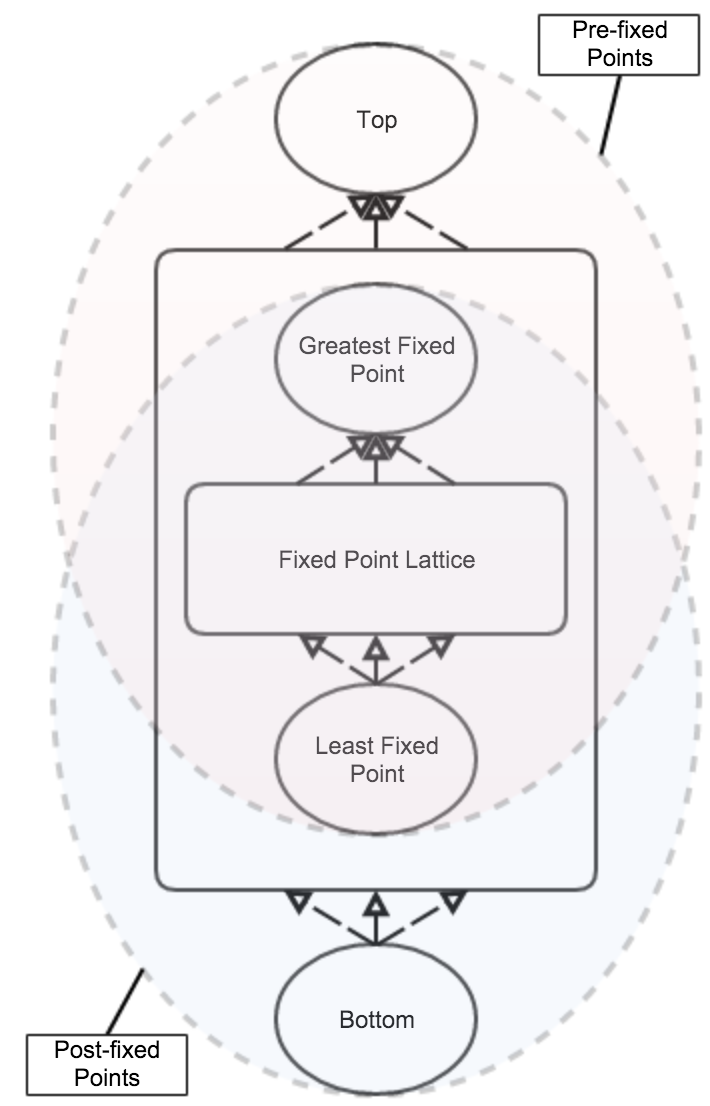
\includegraphics[width=50mm,scale=0.5]{lattice}
\caption{Fixed Point Lattice Induced by Monotone Endofunction}
\label{fig-lattice}
\end{figure}


Thus, this fixed point framework provides a natural definition for recursive sets:
\begin{itemize}
\item[] \textsc{Inductive set on a complete lattice, $L$, with respect to $F:L \mapsto\mathcal{L}$}: 
$$F_{in} = \wedge \{\, T \in\mathcal{L}\,|\, F(T) \subseteq T \,\}$$
\item[] \textsc{Co-inductive set on a complete lattice, $L$, with respect to $F:L \mapsto L$}: 
$$F_{co} = \vee \{\, T \in\mathcal{L}\,|\, T \subseteq F(T) \,\}$$
\end{itemize}

Furthermore, these definitions naturally give rise to the principles of induction and coinduction:
\begin{itemize}
\item[] \textsc{Principle of Induction}: $F(T) \subseteq T \Rightarrow F_{in} \subseteq T$
\item[] \textsc{Principle of Coinduction}: $T \subseteq F(T) \Rightarrow T \subseteq F_{co}$
\end{itemize}

The formal justification for these principles follows immediately from the definition of meet and join.
\begin{proof}
Let $T \in \mathcal{L}$, and suppose $F(T) \subseteq T$. Then $F_{in} \subseteq T$, since $F_{in}$ is a lower bound of all prefixed points.
Similarly, if we suppose $T \subseteq F(T)$, then $T \subseteq F_{co}$, since $F_{co}$ is an upper bound of all postfixed points.
\end{proof}

\subsection{Proof by Rule (Co-)Induction}
We now examine how recursive sets specified by deductive systems may be codified in terms of fixed points. Let $\mathcal{U}$ contain the predicate or relation defined by the deductive system. We encode inference rules as a set $R \subseteq \mathcal{P}(\mathcal{U}) \times \mathcal{U}$ of \textit{ground rules}. Each ground rule $(S,x) \in R$ represents a substitution of a recursive object for the variables in an inference rule, where $S$ is the set of sub-objects corresponding to the premises, from which the object corresponding to the conclusion, $x$ follows. Figure \ref{fig-nat-ground-rules} demonstrates the set encoding of the `Nat' predicate defined in the deductive system of Figure \ref{fig-nat-sys}.

\begin{figure}
\caption{Set Encoding of Inference Rules for Natural Numbers}
\label{fig-nat-ground-rules}
$$\mathcal{U} = \{Z,S,(,)\}^*$$
$$R = \{(\emptyset,Z)\} \cup \{(\{n\},S(n)) : \forall n \in \mathcal{U}\}$$ 
\end{figure}

We simulate the construction of objects with the endofunction $\Phi_R$, called the \textbf{rule functional}, defined over the powerset lattice induced by $\mathcal{U}$ as:
$$\Phi_R(T) = \{\,x \in \mathcal{U} \,|\,\exists (S,x) \in R : S \subseteq T \,\}$$

%The inductive set can be constructed by the following algorithm: starting with $T = \emptyset$, we add to $T$ all objects derivable from $R$ using premises in $T$. In the first iteration only the axiomatically derivable objects are added to $T$; more complex derivations occur in subsequent iterations. This algorithm can be described as the iterative application of an operator $\Phi_R:\mathcal{P}(X) \mapsto \mathcal{P}(X)$, called the \textbf{rule functional}, that takes a set of objects, $T$ and produces the set of objects constructible under $R$ using the objects in $T$ as premises:

%$$\Phi_R(T) = \{\,x \in \mathcal{U} \,|\,\exists (S,x) \in R : S \subseteq T \,\}$$

%For example: the deductive system for the natural numbers in Figure \ref{fig-nat-sys} induces the following rule functional:
%$$\Phi_R(T) = \{Z\} \,\cup\, \{S(N) \,|\, \forall N \in T\} $$

%In this case, it's easy to see how the iterative application of the rule functional constructs the inductive set:
%$$\Phi_R(\emptyset) = \{Z\}$$
%$$\Phi_R(\Phi_R(\emptyset)) = \{Z,S(Z)\}$$
%$$...$$
%$$\Phi_R^n(\emptyset) = \{Z,S(Z),S(S(Z)),...,S(S(S(...S(Z)...))) \text{ (n-1 S's)}\} [\forall n \in \mathbb{N}]$$

%Dually, the construction of the co-inductive set proceeds backwards: we begin with $T = \mathcal{U}$ and, with each iteration, remove all objects whose sub-objects are not in $T$. Remarkably, this algorithm can also be described as the iterative application of $\Phi_R(T)$, although the construction is more difficult to visualize as the rule functional operates on infinite sets at each step. One can imagine that malformed strings such as ``$Z(S(Z(S)...))$" or ``$(S)Z)$" are removed at each step, leaving only those strings of the form $S(S(S(S(...))))$.

%\begin{figure}[h]
%\caption{Construction of the Inductive Set as Traversal of Post-Fixed Points}
%\label{ind-construction}

%$$\emptyset \subseteq \Phi_R(\emptyset) \subseteq \Phi_R(\Phi_R(\emptyset)) \subseteq ... \subseteq \Phi_R^n(\emptyset) \subseteq ... \subseteq \mathbb{N} \supseteq \Phi_R(\mathbb{N})$$

%\end{figure}

The principles of \textbf{rule induction} and \textbf{rule co-induction} can be gleaned from the principles of induction and coinduction by letting $T \equiv \{x \in \mathcal{U} \,| P(x)\} \in \mathcal{P}(\mathcal{U})$, the set induced by an arbitrary predicate $P(x)$ over $\mathcal{U}$ \cite{Pierce2002}:

\begin{itemize}
\item \textsc{Principle of Rule Induction}: $$[\forall (S,x) \in R: (\forall x' \in S: P(x')) \Rightarrow P(x)] \Rightarrow [\forall x \in \mathcal{U}: x \in {\Phi_R}_{in} \Rightarrow P(x)]$$
\item \textsc{Principle of Rule Coinduction}: $$[\forall x \in \mathcal{U}: P(x) \Rightarrow (\exists (S,x) \in R: \forall x' \in S: P(x'))] \Rightarrow [\forall x \in \mathcal{U}: P(x) \Rightarrow x \in {\Phi_R}_{co}]$$
\end{itemize}

\begin{proof}
Let $T$ be the set induced by some arbitrary predicate, $P(x)$.

To prove the principle of rule induction, we must show that $\forall x \in \mathcal{U}: x \in {\Phi_R}_{in} \Rightarrow P(x)$, assuming that $\forall (S,x) \in R: (\forall x' \in S: P(x')) \Rightarrow P(x)$. By applying the definition of both $T$ and $\Phi_R$, we have that:
$$ \forall (S,x) \in R: (\forall x' \in S: x' \in T) \Rightarrow x \in T  \iff$$
$$ \forall (S,x) \in R: S \subseteq T \Rightarrow x \in T \iff$$
$$ \forall x \in \Phi_R(T): x \in T \iff$$
$$ \Phi_R(T) \subseteq T$$

Thus, by the principle of induction, we have that ${\Phi_R}_{in} \subseteq T$. It follows then, that for an arbitrary $x \in {\Phi_R}_{in}$, $x \in T$, or equivalently, $P(x)$.

Similarly, to prove the principle of rule coinduction, we must show $\forall x \in \mathcal{U}: P(x) \Rightarrow x \in {\Phi_R}_{co}$, assuming that $\forall x \in \mathcal{U}: P(x) \Rightarrow (\exists (S,x) \in R: \forall x' \in S: P(x'))$. By applying the definition of both $T$ and $\Phi_R$, we have that: 
$$\forall x \in \mathcal{U}: x \in T \Rightarrow (\exists (S,x) \in R: \forall x' \in S: x' \in T) \iff$$
$$\forall x \in T : (\exists (S,x) \in R: S \subseteq T) \iff$$
$$\forall x \in T: x \in \Phi_R(T) \iff$$
$$T \subseteq \Phi_R(T)$$

Thus, by the principle of coinduction, we have that $T \subseteq {\Phi_R}_{co}$. It follows then, that for any arbitrary $x \in \mathcal{U}$ with $P(x)$, since $x \in T$ by definition of $T$, it follows that $x \in {\Phi_R}_{co}$.

Note that, at first glance, the structure of a coinductive proof seems to be operate dually to an inductive proof: the latter requires a proof by case analysis on each inference rule, whereas the former seemingly requires the satisfaction of just one case. However, this cursory view neglects the fact that each coinductive case incurs a loss of generality by assuming a specific form object form; thus, every inference rule must be analyzed independently to recover generality. One key difference lies in the treatment of axioms: since they lack premises, their respective cases can be omitted.

\end{proof}

We now illustrate how familiar inductive and co-inductive proofs emerge from the machinery of the fixed-point framework. Normally, such proofs proceed without explicit reference to this underlying machinery.

\textbf{Example 1: Proof by Induction} 

We prove the antisymmetry of the $\le$ relation from Figure \ref{fig-less-than-sys}.

\textbf{Antisymmetry Lemma}: $\forall n, m \in \mathbb{N}: (n \le m \wedge m \le n) \Rightarrow n = m$

\begin{proof}[\textsc{Proof}]

We can recognize the lemma as a candidate for a proof by induction by letting:
\begin{itemize}
\item[] $\mathcal{U} \equiv \mathbb{N} \times \mathbb{N}$
\item[] $F_{in} \equiv lfp(\Phi_{\le})$
\item[] $P(n,m) \equiv (m \le n \Rightarrow n = m)$

\end{itemize}

Where, $\Phi_{\le}$ denotes the rule functional induced by the rules of $\le$: 
$$\le \, \equiv \{ (\emptyset ,(Z,n)) \,|\ \forall n \in \mathbb{N} \} \cup \{ (\{ (n,m) \} , (S(n),S(m))) \,|\ \forall n,m \in \mathbb{N} \}$$

Thus, the lemma can be restated as: $\forall (n,m) \in \mathbb{N} \times \mathbb{N}: (n,m) \in F_{in} \Rightarrow P(n,m)$. By the principle of induction, it suffices to perform a proof by rule induction on the derivation of $n \le m$; that is, we must show: $\forall (S,(n,m)) \in \,\le: (\forall (n',m') \in S: P(n',m')) \Rightarrow P(n,m)$.

Let $(S,(n,m)) \in \, \le$. Then $(S,(n,m)) \in \{ (\emptyset ,(Z,m)) \,|\ \forall m \in \mathbb{N} \}$ or $\{ (\{ (n',m') \} , (S(n'),S(m'))) \,|\ \forall (n',m') \in \mathbb{N} \times \mathbb{N} \}$. Thus, an analysis of the ground rules corresponds to a case analysis of each of the inference rules in the deductive system; for each case, we must conclude $P(x)$.

\underline{Case 1}: $(S,(n,m)) \in \{ (\emptyset, (Z, m) \,|\ \forall m \in \mathbb{N} \}$

In this case, $n = Z$. By assumption, we have $m \le Z$; therefore, there is some $S \subseteq \mathbb{N} \times \mathbb{N}$ such that $(S,(m,Z)) \in \, \le$. By inspection of the rules, we observe that, since there is no $y \in \mathbb{N}$ such that $Z = S(y)$, it must be the case that $S = \emptyset$ and $m = Z$. Therefore, $n = m$.

\underline{Case 2}: $(S,(n,m)) \in \{ (\{ (n',m') \} , (S(n'),S(m'))) \,|\ \forall n',m' \in \mathbb{N} \}$

In this case, $(n,m) = (S(n'),S(m'))$ and $(n',m') \in \mathbb{N} \times \mathbb{N}$. In addition, we may assume the inductive hypothesis: $m' \le n' \Rightarrow n' = m'$. By assumption, we have $S(m') \le S(n')$, and, as in the previous case, an inspection of the rules reveals that it must be the case that $m' \le n'$. By the inductive hypothesis, then, we have that $m' = n'$, and so $S(n') = S(m')$.
\end{proof}

It is interesting to note that, rather than perform rule induction on the derivation of $n \le m$, one could alternatively perform rule induction on the derivation of Nat$(n)$ by making the following selections:
\begin{itemize}
\item[] $\mathcal{U} \equiv \{ S,Z,(,) \}^*$
\item[] $F_{in} \equiv \mathbb{N}$
\item[] $P(n) \equiv \forall m \in \mathbb{N}: (n \le m \wedge m \le n) \Rightarrow n = m$
\end{itemize}

\textbf{Example 2: Proof by Co-induction} 

Consider the recursive definitions in Figures \ref{list-sys} and \ref{lex-sys}. The former defines the set of lists constructible from elements of a set $A$, whose elements have a natural, transitive ordering, $\le$. The co-inductive interpretation of this definition yields the set of both finite and infinite lists: the set $A^\omega$. The latter defines a lexicographical ordering on lists, where $hd(\sigma )$ and $tl(\sigma )$ refer to the elements on either side of the `$:$' operator.

\begin{figure}
	\caption{Recursive Definition for $A^\omega$}
	\label{list-sys}
	\centering
	
	
	\vskip 0.2in	
	\AxiomC{}
	\UnaryInfC{nil $\in A^\omega$}
	\RightLabel{\scriptsize(nil)}
	\DisplayProof 		
	\hskip 0.3in		
	\AxiomC{$\tau \in A^\omega$}
	\AxiomC{$a \in A$}
	\BinaryInfC{$a:\tau \in A^\omega$}
	\RightLabel{\scriptsize(cons)}
	\DisplayProof
\end{figure}

\begin{figure}
	\caption{Recursive Definition for $\le_{L}$}
	\label{lex-sys}
	\centering

	\vskip 0.2in		
	\AxiomC{}
	\UnaryInfC{$nil \le_{L} \sigma$}
	\RightLabel{\scriptsize($nil$)}
	\DisplayProof	
	\hskip 0.2in		
	\AxiomC{$hd(\sigma ) \le hd(\tau )$}
	\AxiomC{$hd(\sigma ) = hd(\tau ) \Rightarrow tl(\sigma ) \le_{L} tl(\tau )$}
	\BinaryInfC{$\sigma \le_{L} \tau$}
	\RightLabel{\scriptsize($cons$)}
	\DisplayProof
	
\end{figure}

We now prove the transitivity of lexicographical ordering for infinite lists, as stated by the following lemma:

\textbf{Transitivity Lemma}: $\forall \sigma, \tau \in A^\omega: (\exists \rho \in A^\omega: \sigma \le_{L} \rho \le_{L} \tau) \Rightarrow (\sigma \le_{L} \tau)$ 

\begin{proof}[Proof:]
We can recognize the statement as a candidate for a proof by rule co-induction by letting:
\begin{itemize}
\item[] $\mathcal{U} \equiv A^\omega \times A^\omega$
\item[] $P(\sigma,\tau) \equiv \exists \rho \in A^\omega: \sigma \le_{L} \rho \le_{L} \tau$
\item[] $F_{co} \equiv gfp(\Phi_{\le_{L}})$
\end{itemize}

Where $\Phi_{\le_{L}}$ is the rule functional induced by the ground rules:
$$\le_{L} \equiv \{~( ~\{ (tl(\sigma),tl(\tau)) \,|\ hd(\sigma) = hd(\tau) \}, (\sigma,\tau)) \,|\ \forall (\sigma,\tau) \in A^\omega \times A^\omega: hd(\sigma) \le hd(\tau) \} ~\cup~ \{(\emptyset,(nil,\sigma)) \,|\ \forall \sigma \in A^\omega \}$$

Thus, the lemma can be restated as: $\forall (\sigma,\tau) \in \mathcal{U}: P(\sigma,\tau) \Rightarrow (\sigma,\tau) \in {\Phi_{\le_{L}}}_{co}$. By the principle of co-induction, it suffices to perform a proof by rule co-induction on the derivation of $\sigma \le_{L} \tau$; that is, we must show: $\forall (\sigma,\tau) \in \mathcal{U}: P(\sigma,\tau) \Rightarrow \exists (S,(\sigma,\tau)) \in \le_{L}: \forall (\sigma',\tau') \in S: P(\sigma',\tau')$. 

Let $(\sigma,\tau) \in A^\omega \times A^\omega$ be such that $\exists \rho \in A^\omega: \sigma \le_{L} \rho \le_{L} \tau$, i.e., the \textbf{coinductive hypothesis}. We must find a ground rule $(S,(\sigma,\tau)) \in \le_{L}$ such that $\forall (\sigma',\tau') \in S: P(\sigma',\tau')$. As explained earlier, this corresponds to a case analysis of the ground rules, where each case requires the construction of the premises, $S$, and a proof of $P(x)$ for each $x \in S$, in addition to any side conditions:

\underline{Case 1}: $(S,(\sigma,\tau)) \in \{(\emptyset,(nil,\sigma)) \,|\ \forall \sigma \in A^\omega \}$

In this case we have $\sigma = nil$, and so the proof follows immediately since $(\emptyset, (nil,\tau)) \in \le_{L}$. As this case carried no proof obligations, it could have been omitted.

\underline{Case 2}: $(S,(\sigma,\tau)) \in \{~( ~\{ (tl(\sigma),tl(\tau)) \,|\ hd(\sigma) = hd(\tau) \}, (\sigma,\tau)) \,|\ \forall (\sigma,\tau) \in A^\omega \times A^\omega: hd(\sigma) \le hd(\tau) \}$

In this case, we have three proof obligations:
\begin{itemize}
\item[] \textbf{Construction of Premises $S$}: $(\{(tl(\sigma),tl(\tau)) \,| hd(\sigma) = hd(\tau)\},(\sigma,\tau)) \in \,\le_{L}$
\item[] \textbf{Proof of Side Condition}: $hd(\sigma) \le hd(\tau)$
\item[] \textbf{Show Property on Premises}: $\forall (\sigma',\tau') \in \{(tl(\sigma),tl(\tau)) \,| hd(\sigma) = hd(\tau)\}: P(\sigma',\tau')$
\end{itemize}

The side condition follows immediately from the coinductive hypothesis, which gives us $hd(\sigma) \le hd(\rho) \le hd(\tau)$, and the transitivity of $\le$.

Now, we consider two subcases: $hd(\sigma) = hd(\tau)$ and $hd(\sigma) \not= hd(\tau)$. The latter case is immediately proven by the fact that there are no premises. 

Thus, suppose $hd(\sigma) = hd(\tau)$. Then we have $hd(\sigma) = hd(\rho)$ and $hd(\rho) = hd(\tau)$. By inspection of the rules $\le_{L}$ in the coinductive hypothesis, and the fact that neither $\sigma$ nor $\tau$ can be $nil$, since $hd(nil)$ is undefined, it follows that $hd(\sigma) = hd(\rho) \Rightarrow tl(\sigma) \le_{L} tl(\rho)$ and $hd(\rho) = hd(\tau) \Rightarrow tl(\rho) \le_{L} tl(\tau)$. Thus, we have $tl(\sigma) \le_{L} tl(\rho) \le_{L} tl(\tau)$, satisfying the final proof obligation: $\exists \rho \in A^\omega: tl(\sigma) \le_{L} \rho \le_{L} tl(\tau)$.

\end{proof}


